The problem of substituting fluorescence labeling with \textit{in silico} prediction solved in thesis is a step towards a general goal of the project within Merck KGaA oriented towards predicting cell stability and productivity. Instead of a usual feature analysis of sizes of cell organelles, their fluorescence intensities and quantities, one can incorporate feauture representations created by UNet directly into the pipeline for productivity predictions that uses assay features as its inputs (see Figure \ref{fig:productivity-fluroescence}).
\begin{figure}[htb]
	\begin{center}
		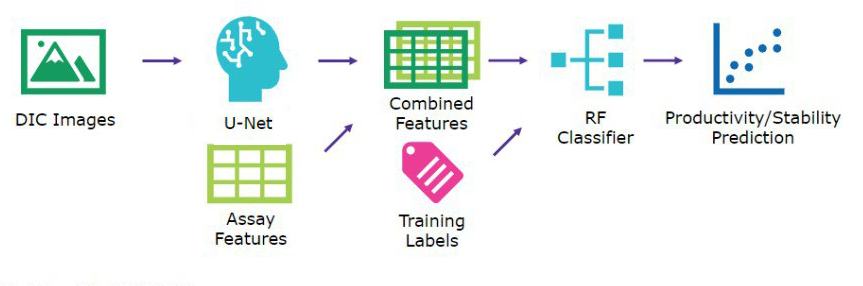
\includegraphics[width=\linewidth]{bilder/unet-embeddings/producitvity.png}
		\caption{Predicting productivity with fluorescence data incorporated}
		\label{fig:productivity-fluroescence}
	\end{center}
\end{figure}

Meaning that instead of training a model directly on assay features that are potentially providing information to predict future cell stability, one could combine them with the embeddings of a UNet model. Embeddings represent a rich representation of cells in DIC that has information on features needed for detecting cell organelles, therefore they might include other useful knowledge that was not analysed in the lab before and can be potentially useful for cell analysis. Most probably assay features will be combined with several UNet embeddings, as several different models were trained to predict different targets, however it would be possible to train a signle UNet model that would predict all targets at once, that will ensure even more informationally rich embeddings. Afterwards, with the help of random forest classifier productivity and stability rates can be derived. 

This approach has a strong theorectical portential behind it and requires acquiring stability and productivity data first to have a proof of concept. Since data acquisition in for this task requires more than 9 months, therefore the experiments could not be held within the scope of this work, but will be researched in the nearest future.